\documentclass[a4paper,14pt]{article}
\usepackage{float}
\usepackage{extsizes}
\usepackage{amsmath}
\usepackage{amssymb}
\everymath{\displaystyle}
\usepackage{geometry}
\usepackage{fancyhdr}
\usepackage{multicol}
\usepackage{graphicx}
\usepackage[brazil]{babel}
\usepackage[shortlabels]{enumitem}
\usepackage{cancel}
\usepackage{textcomp}
\usepackage{array} % Para melhor formatação de tabelas
\usepackage{longtable}
\usepackage{booktabs}  % Para linhas horizontais mais bonitas
\usepackage{float}   % Para usar o modificador [H]
\usepackage{caption} % Para usar legendas em tabelas

\columnsep=2cm
\hoffset=0cm
\textwidth=8cm
\setlength{\columnseprule}{.1pt}
\setlength{\columnsep}{2cm}
\renewcommand{\headrulewidth}{0pt}
\geometry{top=1in, bottom=1in, left=0.7in, right=0.5in}

\pagestyle{fancy}
\fancyhf{}
\fancyfoot[C]{\thepage}

\begin{document}
	
	\noindent\textbf{6FMA39 - Matemática} 
	
	\begin{center}Adição e subtração e representação na reta (Versão estudante)
	\end{center}
	
	\noindent\textbf{Nome:} \underline{\hspace{10cm}}
	\noindent\textbf{Data:} \underline{\hspace{4cm}}
	
	%\section*{Questões de Matemática}	
    \begin{multicols}{2}
    	\noindent Somar um número inteiro positivo a um número inteiro $x$ significa "andar", no mesmo sentido de orientação da reta, tantas unidades quantas forem esse número. \\
    	Somar um número inteiro negativo a um número inteiro $x$ significa "andar", em sentido contrário à orientação da reta, tantas unidades quantas forem o módulo desse número.
    	Para todo inteiro $x$, temos $x + 0 = x$.
    	\noindent\textsubscript{~---------------------------------------------------------------------------}
    	\begin{enumerate}
    		\item Representar na reta:
    		\begin{enumerate}[a)]
    			\item $x + 6$ \\
    			\noindent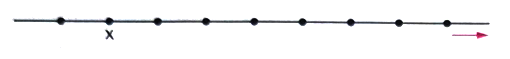
\includegraphics[width=1.1\linewidth]{imagens_6FMA39/imagem1}
    			\\
    			\item $m - 4$ \\
    			\noindent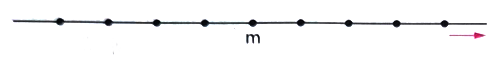
\includegraphics[width=1.1\linewidth]{imagens_6FMA39/imagem2}
    			\\
    			\item $y + 0$ \\
    			\noindent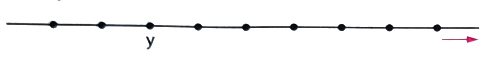
\includegraphics[width=1.1\linewidth]{imagens_6FMA39/imagem3}
    			\columnbreak
    			\item $k + 5$ \\
    			\noindent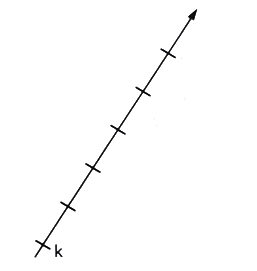
\includegraphics[width=1.1\linewidth]{imagens_6FMA39/imagem4}
    			\\
    			\item $\ell - 3$ \\
    			\noindent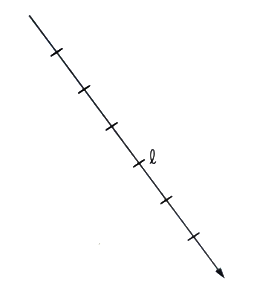
\includegraphics[width=1.1\linewidth]{imagens_6FMA39/imagem5}
    			\newpage
    			\item $g + 3$ \\
    			\noindent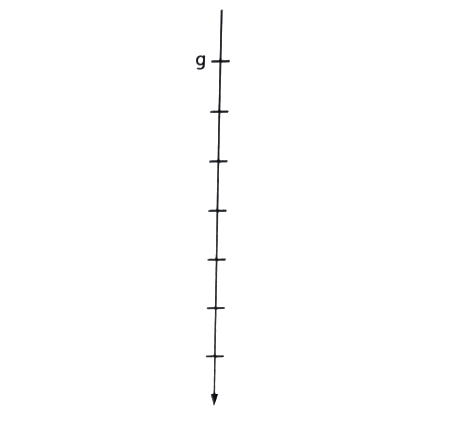
\includegraphics[width=1.1\linewidth]{imagens_6FMA39/imagem6}
    			\\
    		\end{enumerate}
    		\item Efetuar, colocando na reta o primeiro número e a soma, como visto na definição.
    		\begin{enumerate}[a)]
    			\item 2 + 3 \\\\\\
    			\item -3 + 5 \\\\\\
    			\item -4 + 4 \\\\\\
    			\item -6 + 2 \\\\\\
    		\end{enumerate}
    		\item Efetuar:
    		\begin{enumerate}[a)]
    			\item 8 + 5 \\\\\\\\
    			\item -15 + 6 \\\\\\\\
    			\item 0 + 12 \\\\\\\\
    			\item -18 + 18 \\\\\\\\
    			\item 25 - 32 \\\\\\\\
    		\end{enumerate}
    		\item Efetuar:
    		\begin{enumerate}[a)]
    			\item -20 +(-2) \\\\\\
    			\item -41 + (-7) \\\\\\
    			\item 31 +(-31) \\\\
    			\item -50 +(-10) \\\\
    			\item 34 +(-4) \\\\\\
    		\end{enumerate}
    	\end{enumerate}
    \end{multicols}
\end{document}